%%%%%%%%%%%%%%%%%%%%%%%%%%%%%%%%%%%%%%%%%
% baposter Landscape Poster
% LaTeX Template
% Version 1.0 (11/06/13)
%
% baposter Class Created by:
% Brian Amberg (baposter@brian-amberg.de)
%
% This template has been downloaded from:
% http://www.LaTeXTemplates.com
%
% License:
% CC BY-NC-SA 3.0 (http://creativecommons.org/licenses/by-nc-sa/3.0/)
%
%%%%%%%%%%%%%%%%%%%%%%%%%%%%%%%%%%%%%%%%%

%----------------------------------------------------------------------------------------
%	PACKAGES AND OTHER DOCUMENT CONFIGURATIONS
%----------------------------------------------------------------------------------------

\documentclass[landscape,a0paper,fontscale=0.35]{baposter} % Adjust the font scale/size here
\usepackage{tabu}
\usepackage{graphicx} % Required for including images
\graphicspath{{figures/}} % Directory in which figures are stored
\usepackage[ngerman]{babel}
\usepackage{amsmath} % For typesetting math
\usepackage{amssymb} % Adds new symbols to be used in math mode
\usepackage[utf8]{inputenc}
\usepackage{booktabs} % Top and bottom rules for tables
\usepackage{enumitem} % Used to reduce itemize/enumerate spacing
\usepackage{helvet} % Use the Palatino font
\usepackage{url}
\usepackage{csquotes}
\usepackage{tabularx}
\renewcommand{\familydefault}{\sfdefault}
\usepackage[font=small,labelfont=bf]{caption} % Required for specifying captions to tables and figures

\usepackage{multicol} % Required for multiple columns
\setlength{\columnsep}{1.5em} % Slightly increase the space between columns
\setlength{\columnseprule}{0mm} % No horizontal rule between columns

\usepackage{tikz} % Required for flow chart
\usetikzlibrary{shapes,arrows} % Tikz libraries required for the flow chart in the template

\newcommand{\compresslist}{ % Define a command to reduce spacing within itemize/enumerate environments, this is used right after \begin{itemize} or \begin{enumerate}
\setlength{\itemsep}{1pt}
\setlength{\parskip}{0pt}
\setlength{\parsep}{0pt}
}

\definecolor{lightblue}{rgb}{0.145,0.6666,1} % Defines the color used for content box headers

\begin{document}

\begin{poster}
{
headerborder=closed, % Adds a border around the header of content boxes
colspacing=1em, % Column spacing
bgColorOne=white, % Background color for the gradient on the left side of the poster
bgColorTwo=white, % Background color for the gradient on the right side of the poster
borderColor=black, % Border color
headerColorOne=gray, % Background color for the header in the content boxes (left side)
headerColorTwo=gray, % Background color for the header in the content boxes (right side)
headerFontColor=white, % Text color for the header text in the content boxes
boxColorOne=white, % Background color of the content boxes
textborder=roundedleft, % Format of the border around content boxes, can be: none, bars, coils, triangles, rectangle, rounded, roundedsmall, roundedright or faded
eyecatcher=true, % Set to false for ignoring the left logo in the title and move the title left
headerheight=0.1\textheight, % Height of the header
headershape=rectangle, % Specify the rounded corner in the content box headers, can be: rectangle, small-rounded, roundedright, roundedleft or rounded
headerfont=\Large\bf\textsc, % Large, bold and sans serif font in the headers of content boxes
%textfont={\setlength{\parindent}{1.5em}}, % Uncomment for paragraph indentation
linewidth=2pt % Width of the border lines around content boxes
}
%----------------------------------------------------------------------------------------
%	TITLE SECTION 
%----------------------------------------------------------------------------------------
%
{
\includegraphics[height=6em]{favicon.png}} % First university/lab logo on the left
{\fontsize{32}{32} \textbf{\textsc{Implementation of an Invitation Management System}}\vspace{0.5em}} % Poster title 
{\textsc{\{ Sidney Kuyateh, Steffen Walter, Lukas Priester, Lukas Schnaithmann \} \hspace{12pt} Invitation-Factory}} % Author names and institution
{
\includegraphics[height=7em]{gobuffalo_logo.png}} % Second university/lab logo on the right

%	Einleitung


\headerbox{Einleitung}{name=objectives,column=0,row=0}{

Im Rahmen des Moduls Softwareengineering sollte ein Programm entworfen und ausgearbeitet werden. Für das Entwickeln dieses Programms gab es mehrere Anforderungen, die zu beachten waren.

	\begin{enumerate}\compresslist %chktex 1
	\item Es soll nach Scrum entwickelt werden
	\item Das Programm sollte am Ende verkaufsfähig sein
	\item Unit-Tests waren zu implementieren
	\item Die Umsetzung der durch die Referate vermittelten Inhalte
	\end{enumerate}
}

%	Die Idee

\headerbox{Die Idee}{name=results,column=1,span=2,row=0,}
{
	\begin{multicols}{2}
		Die Idee entstand im Rahmen einer Teamsitzung. Ziel war es, den Menschen etwas zu bieten, was gebraucht wird.
		
		So entstand die Idee einer Webanwendung zur Verwaltung von Einladungen. Das Programm soll dem Anwender helfen seine Einladungen schneller und effizienter zu verschicken. Die Abbildung~\ref{Ideenfindung} zeigt einen Ausschnitt des ersten Entwurfs. Nachlesen kann man diesen auch hier:\\ \url{https://github.com/stuttgart-dhbw/com.dhbw.team3/wiki/Ideenfindung}\\
	
		\begin{center}
			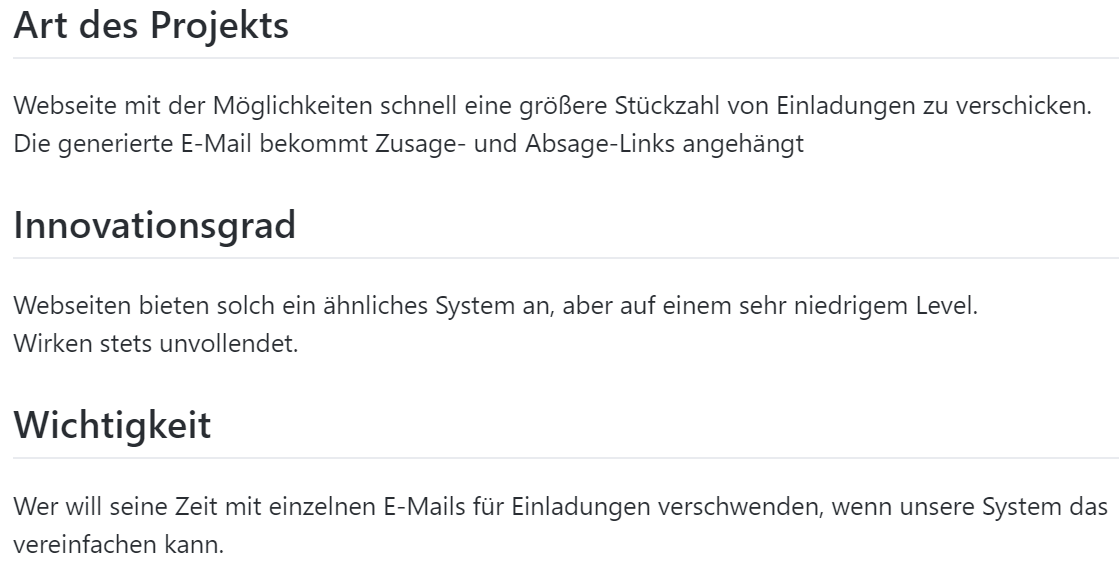
\includegraphics[width=0.69\linewidth]{Ideenfindung_Kleiner.PNG}
			\captionof{figure}{Ideenfindung im Wiki auf GitHub}\label{Ideenfindung}
		\end{center}
	

	\end{multicols}
	
}


\headerbox{Sicherheitserwägungen}{name=introduction,column=3,row=0,span=1}{

	Folgende Maßnahmen sind implementiert um die Sicherheit des Anwendungsservers, des Webservers, des Mailservers und der Datenbank für die Benutzer und Administratoren auf eine möglichst hohe Ebene zu heben.
	
	Es ist ein NGINX Server installiert, welcher als erster Kontaktpunkt für jegliche http Anfragen dient und diese ggf.\ weiterleitet. Dieser ist derart konfiguriert, dass er den Ansprüchen von Mozillas Observatory mehr als gerecht wird. Hierfür sind sehr strenge Sicherheitsvorkehrungen implementiert.\\ Genaueres zeigt Abbildung~\ref{Obervatory} und kann hier nachgelesen werden: \url{https://observatory.mozilla.org/analyze/invitation-factory.tk}
	
	\begin{center}
		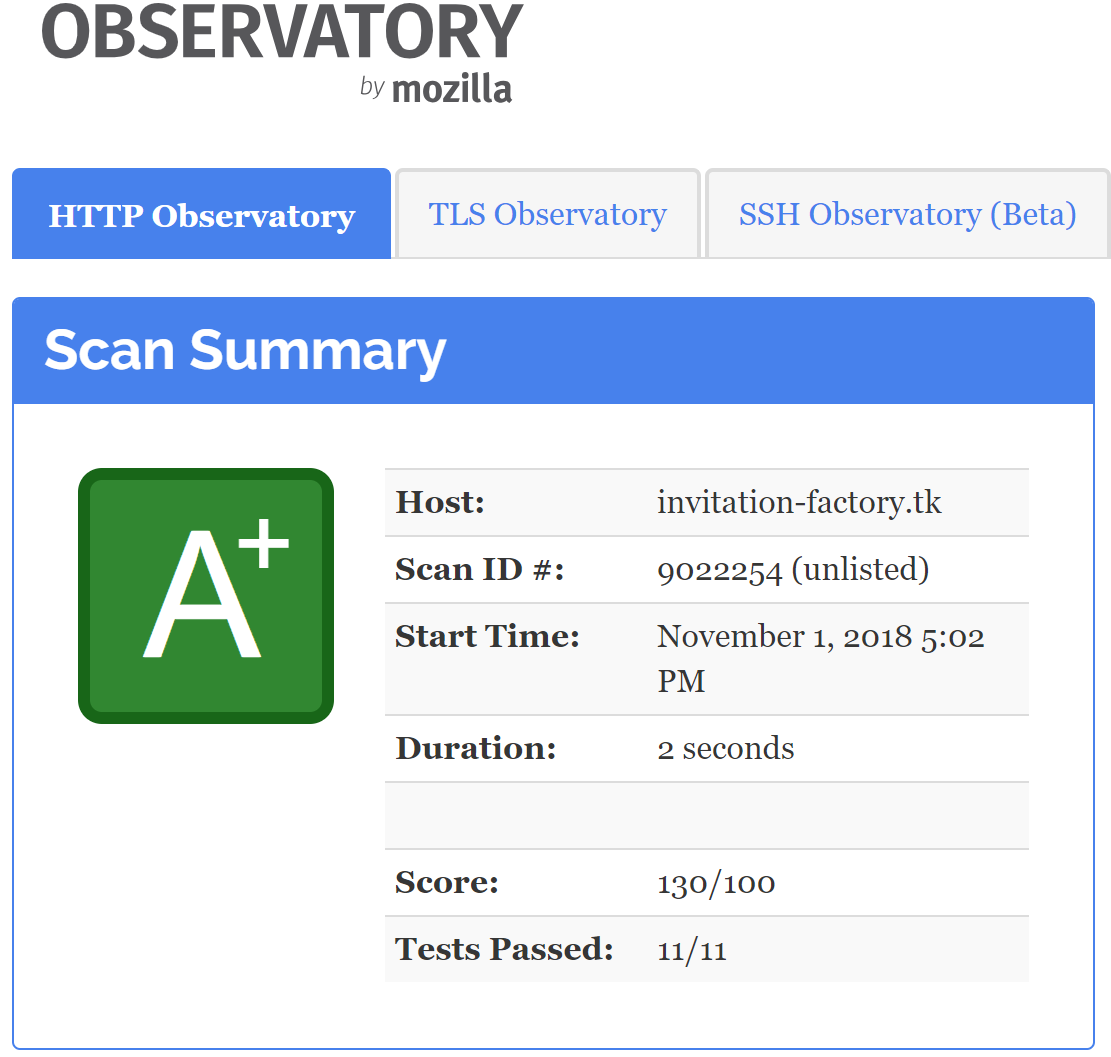
\includegraphics[width=0.45\linewidth]{Observatory.PNG}
		\captionof{figure}{Domain Überprüfung}\label{Obervatory}
	\end{center}

	Als Mailserver kommt Postfix zum Einsatz. Neben einer möglichst sicheren Konfiguration liegt zusätzlich ein Augenmerk auf den E-Mails, welche von diesem Server versendet werden. Ziel ist es die E-Mails nicht von einem Spamfilter abfangen zulassen. Um dies zu erreichen musste dafür gesorgt werden, dass die Serveranwendung den Mails entsprechende Header zufügt, dass die Postfix Konfiguration entsprechend eingestellt wird und es mussten entsprechende DNS Einträge gemacht werden. Zum Test der Konfigurationen wird ein Werkzeug namens Mail-Tester verwendet, bei dem der Postfix Server mit Bestnote abschießt. Das Ergebnis wird in Abbildung~\ref{E-Mail_Tester} dargestellt und kann hier eingesehen werden:
	
	\url{https://www.mail-tester.com/test-foxmj}.

	\begin{center}
		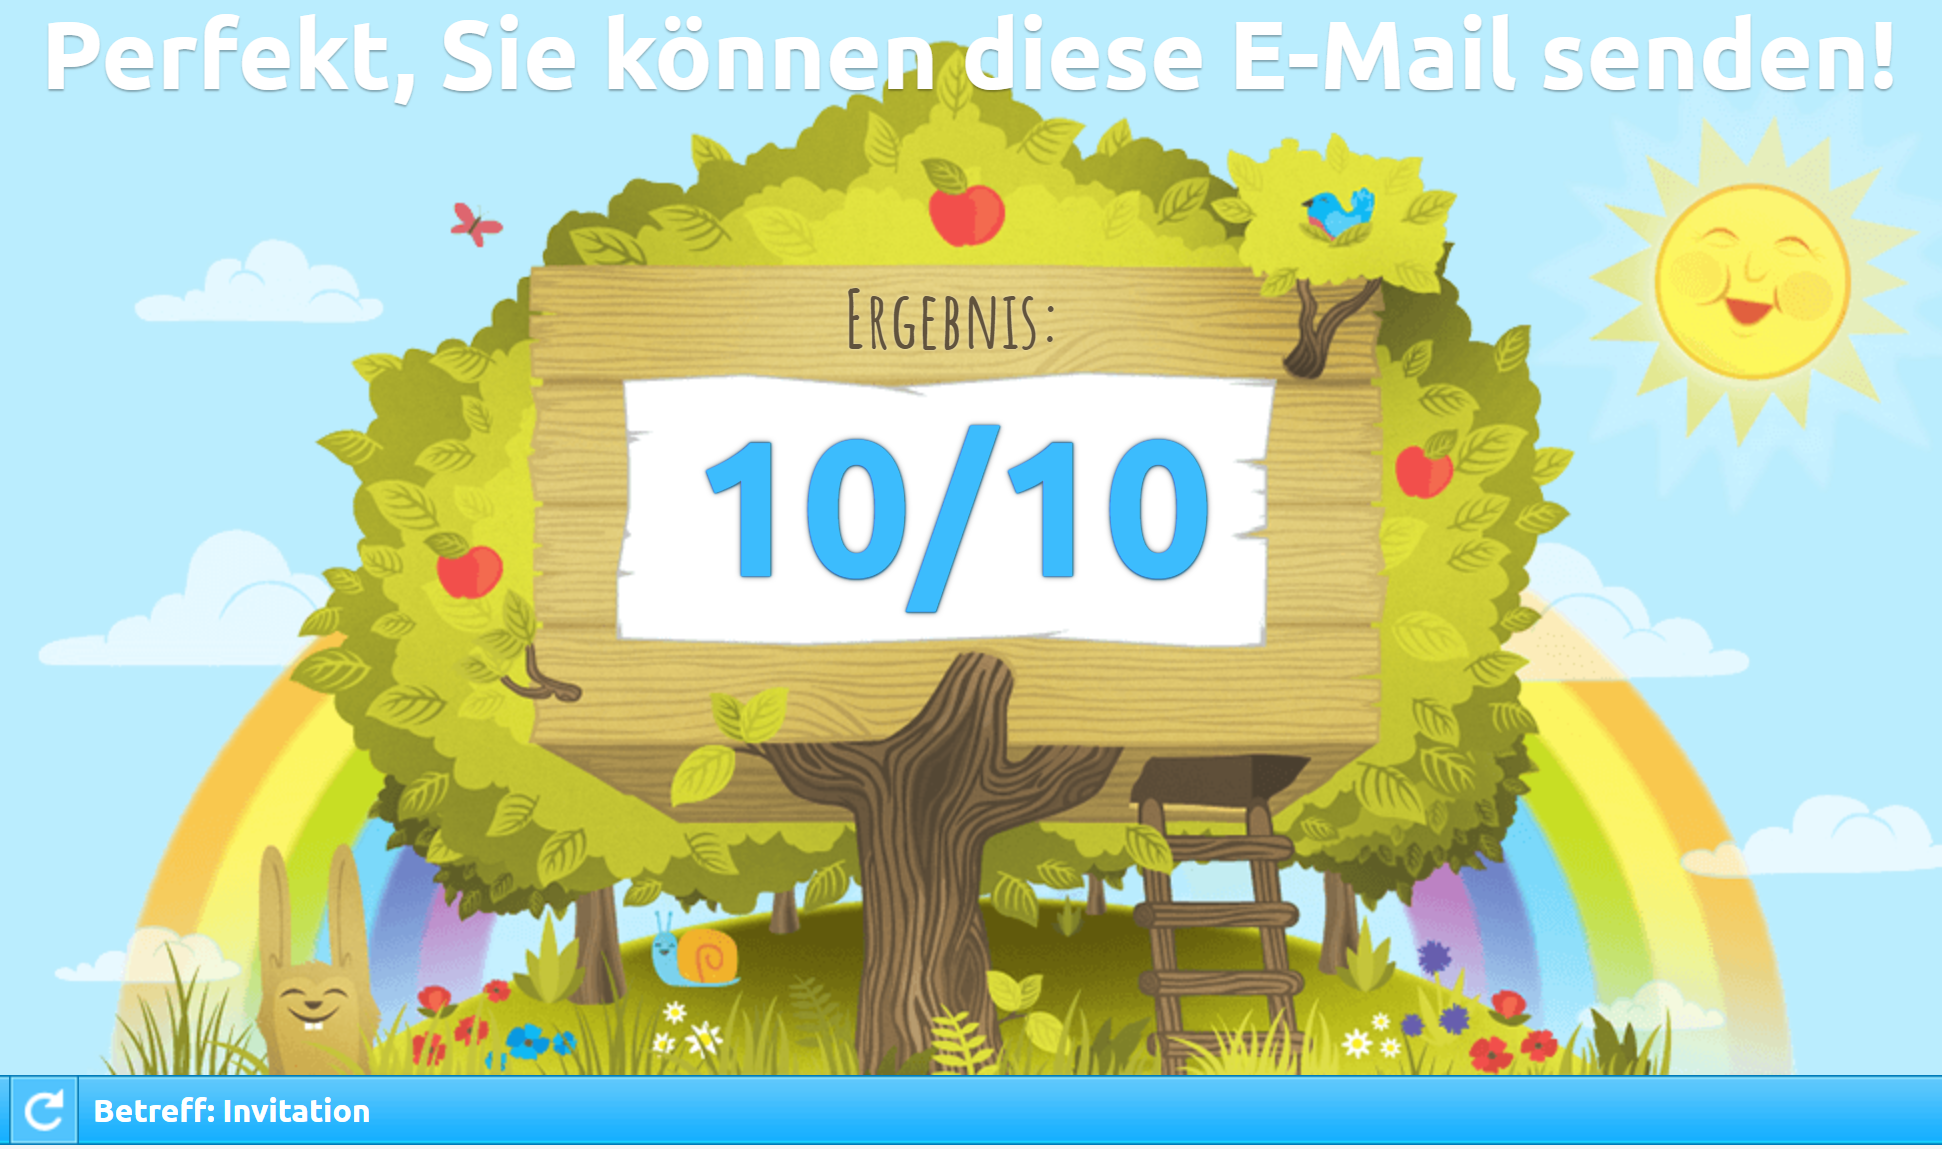
\includegraphics[width=0.5\linewidth]{E-Mail_test.PNG}
		\captionof{figure}{Test um verschickte E-Mail zu überprüfen}\label{E-Mail_Tester}
	\end{center}

	Die Webanwendung hört nur auf einen lokalen Port und wird über den NGINX Server der Außenwelt zur Verfügung gestellt.
	
	Die Transportsicherheit wird also durch den NGINX Server gewährleistet, welcher mit einem Wildcard Let's Encrypt Zertifikat abgesichert ist.
	
	Benutzerpasswörter werden mit dem bcrypt Algorithmus gehasht und nicht im Klartext in der Datenbank abgelegt.
	
	Die Anmeldung auf dem Server ist ausschließlich über SSH und RSA public/private Keys möglich. 
	\vspace{1.2em}
}

%	Projektverlauf

\headerbox{Projektverlauf}{name=method,column=0,below=results,span=2,aligned=references}
{ % This block's bottom aligns with the bottom of the conclusion block
	Bei diesem Projekt wird viel Wert auf die agile Projektentwicklung gelegt. Hierfür wird die Idee von Scrum genutzt, wozu auch die Abbildung~\ref{Scrumboard} einen Einblick in das Scrumboard geben soll. 
	\begin{center}
		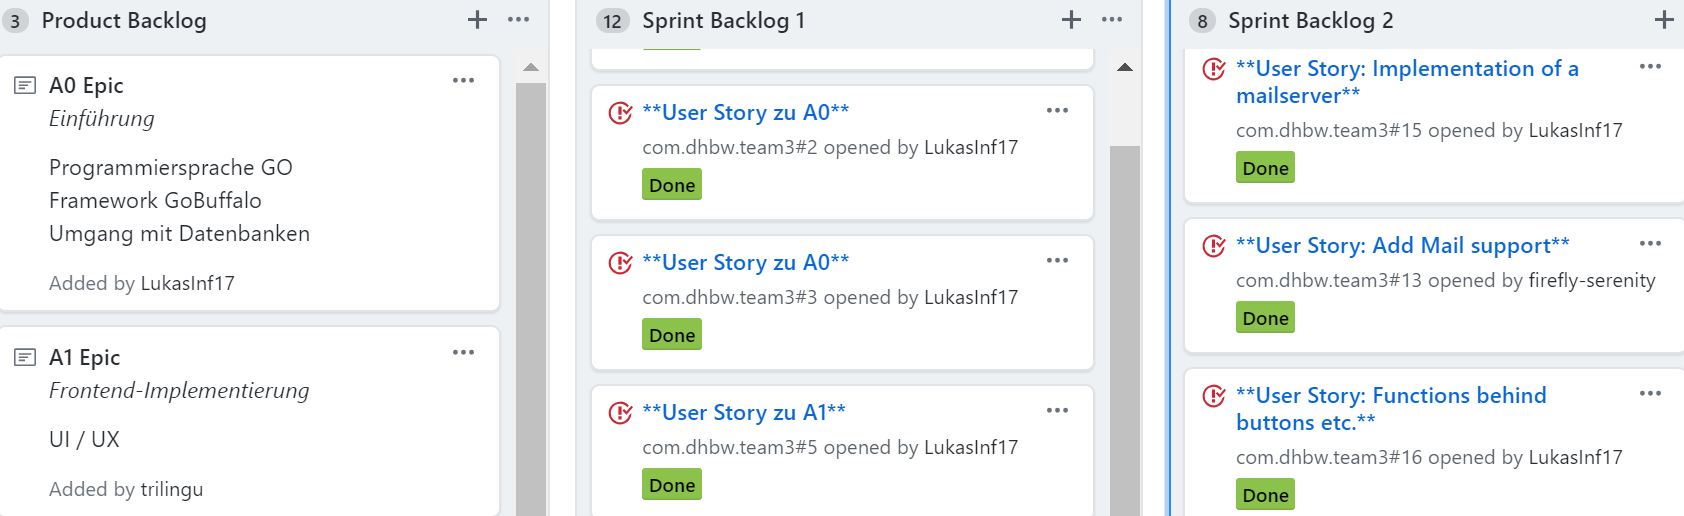
\includegraphics[width=0.8\linewidth]{Scrum_Board_GitHub3.PNG}
		\captionof{figure}{Scrumboard auf GitHub}\label{Scrumboard}
	\end{center}

	Das Projekt belief sich auf einen Zeitraum von 2 Monaten. Dieser wird in 3 Sprints eingeteilt. Dabei entsteht durch den Product Owner und dem Entwicklerteam für jeden Sprint User Stories, die ausgearbeitet und verteilt werden.

	Die nachfolgende Abbildung~\ref{Gantt_Diagramm} soll den Zeitraum mit den Sprints und ihren jeweiligen Aufgaben zeigen.
	\begin{center}
		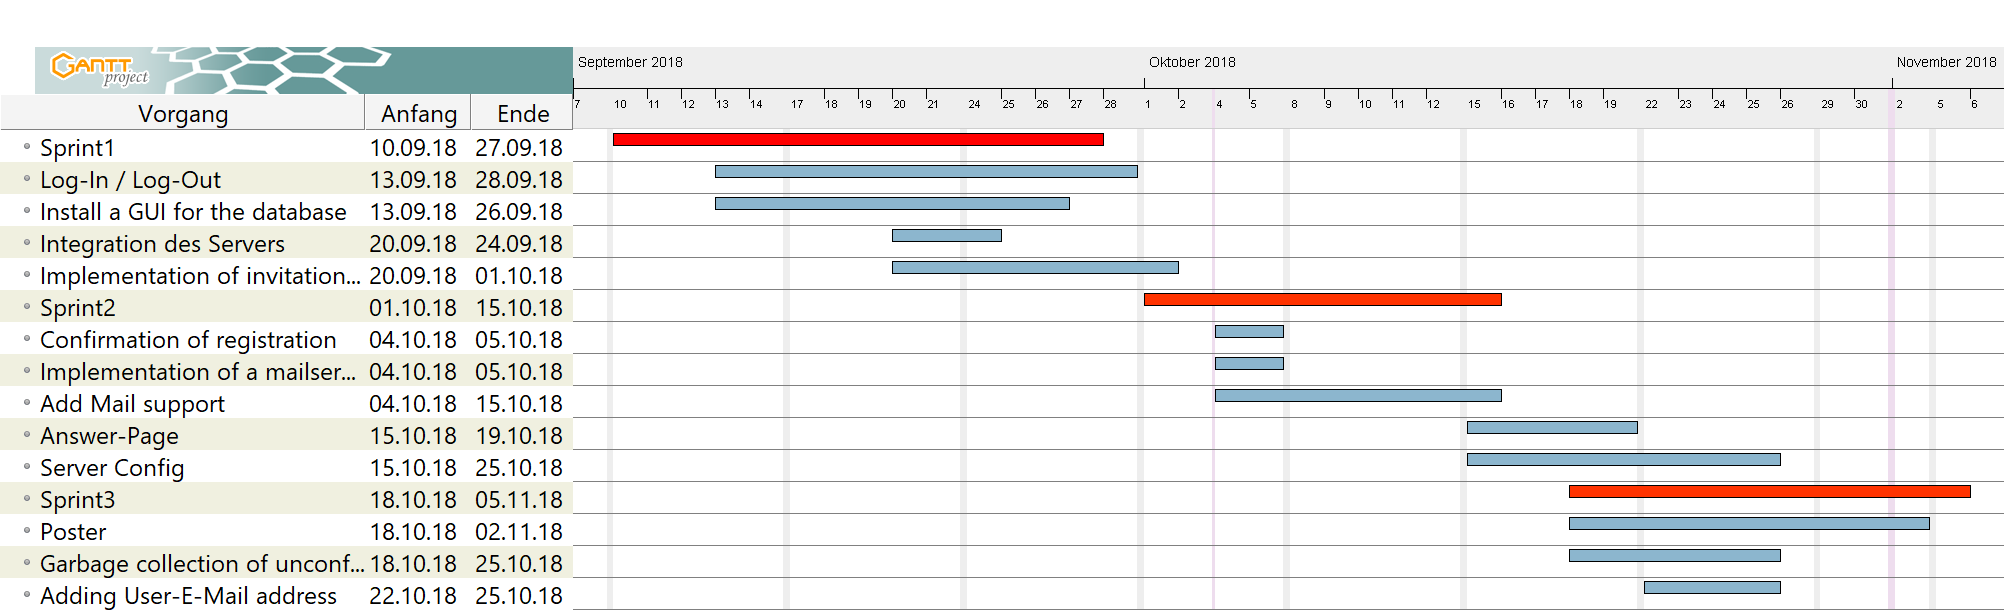
\includegraphics[width=0.82\linewidth]{GanttDiagramm1.PNG}
		\captionof{figure}{GanttDiagramm}\label{Gantt_Diagramm}
	\end{center}
}

%	Methode

\headerbox{Methode}{name=results2,column=2,span=1,aligned=method}
{
	Zur Realisierung des Projektes kam das Framework \enquote{gobuffalo} zum Einsatz. Dabei handelt es sich um eine Umgebung, die es sich zum Ziel gemacht hat, eine Webapplikation unter Verwendung der Programmiersprache GO, möglichst schnell und einfach entwickeln zu können. Zum Einsatz kommen neben GO noch Technologien wie JavaScript, HTML5, CSS und weitere. Die Kernfunktionen von gobuffalo werden in Tabelle~\ref{features} dargestellt.
	\begin{center}
		\begin{tabular}{p{4cm}p{4cm}}
			\toprule
			\textbf{Routing} & \textbf{Templating} \\
			\midrule
			Gorilla toolkit for powerful routing & Plush toolkit for a rails-like HTML templating \\
			\midrule
			\textbf{Buffalo toolkit} & \textbf{Testing} \\
			\midrule
			Buffalo toolkit generates the application,\newline just needed to implement the logics & Define all your test suites and run them from a single command\\
			\bottomrule
		\end{tabular}
	\captionof{table}{Kernfunktionen von gobuffalo}\label{features}
	\end{center}
}

%	Ausblick

\headerbox{Ausblick}{name=ausblick,column=2,span=1,below=results2}
{
	Durch die Umsetzung des aus der Idee heraus geplanten Projekts konnten die Grundfunktionen implementiert werden. Es sind einige zusätzliche Funktionen denkbar, die das Projekt verbessern bzw.\ erweitern könnten.\\
	Die Software ist unter die GPLv3 Lizenz gestellt und somit bietet es die Möglichkeit, dass eine Community gemeinschaftlich an der Weiterentwicklung mitwirken kann.

	Denkbar für die Zukunft sind etwa Funktionen wie die Integration von Facebook, WhatsApp und Co., um auf modernere Kommunikationswege einzugehen.
}

%	Ergebnis

\headerbox{Ergebnis}{name=conclusion,column=0,span=3,row=1,below=method,above=bottom}
{
	\begin{multicols}{3}
		Das Ergebnis dieses Projekts ist mehr als zufriedenstellend. Die Webseite \url{invitation-factory.tk} bietet den Anwendern genau das, was sie wollen. Es bietet ihnen die Möglichkeit Einladungen an Freunde,Familie oder Kollegen zu verschicken, ohne großen Aufwand. Nach einer erfolgreichen Registrierung ist es dem Anwender möglich eine Einladung mit dem gleichen Textinhalt an mehrere Personen zeitgleich zu versenden.
		
		Ein Extra, dass von anderen unterscheiden soll ist die Statusüberprüfung. Der Anwender hat dadurch die Möglichkeit den Status seiner Gäste einzusehen. Es wird ihm also eine separate Seite an angeboten, auf der er schauen kann welcher Gast zu-,abgesagt oder sich noch nicht entschieden hat.
		
		Die Webseite ist anwenderfreundlich und vor allem auch effizient. In Abbildung~\ref{page_sample} wird exemplarisch die Erstellung einer Einladung dargestellt.

		\begin{center}
			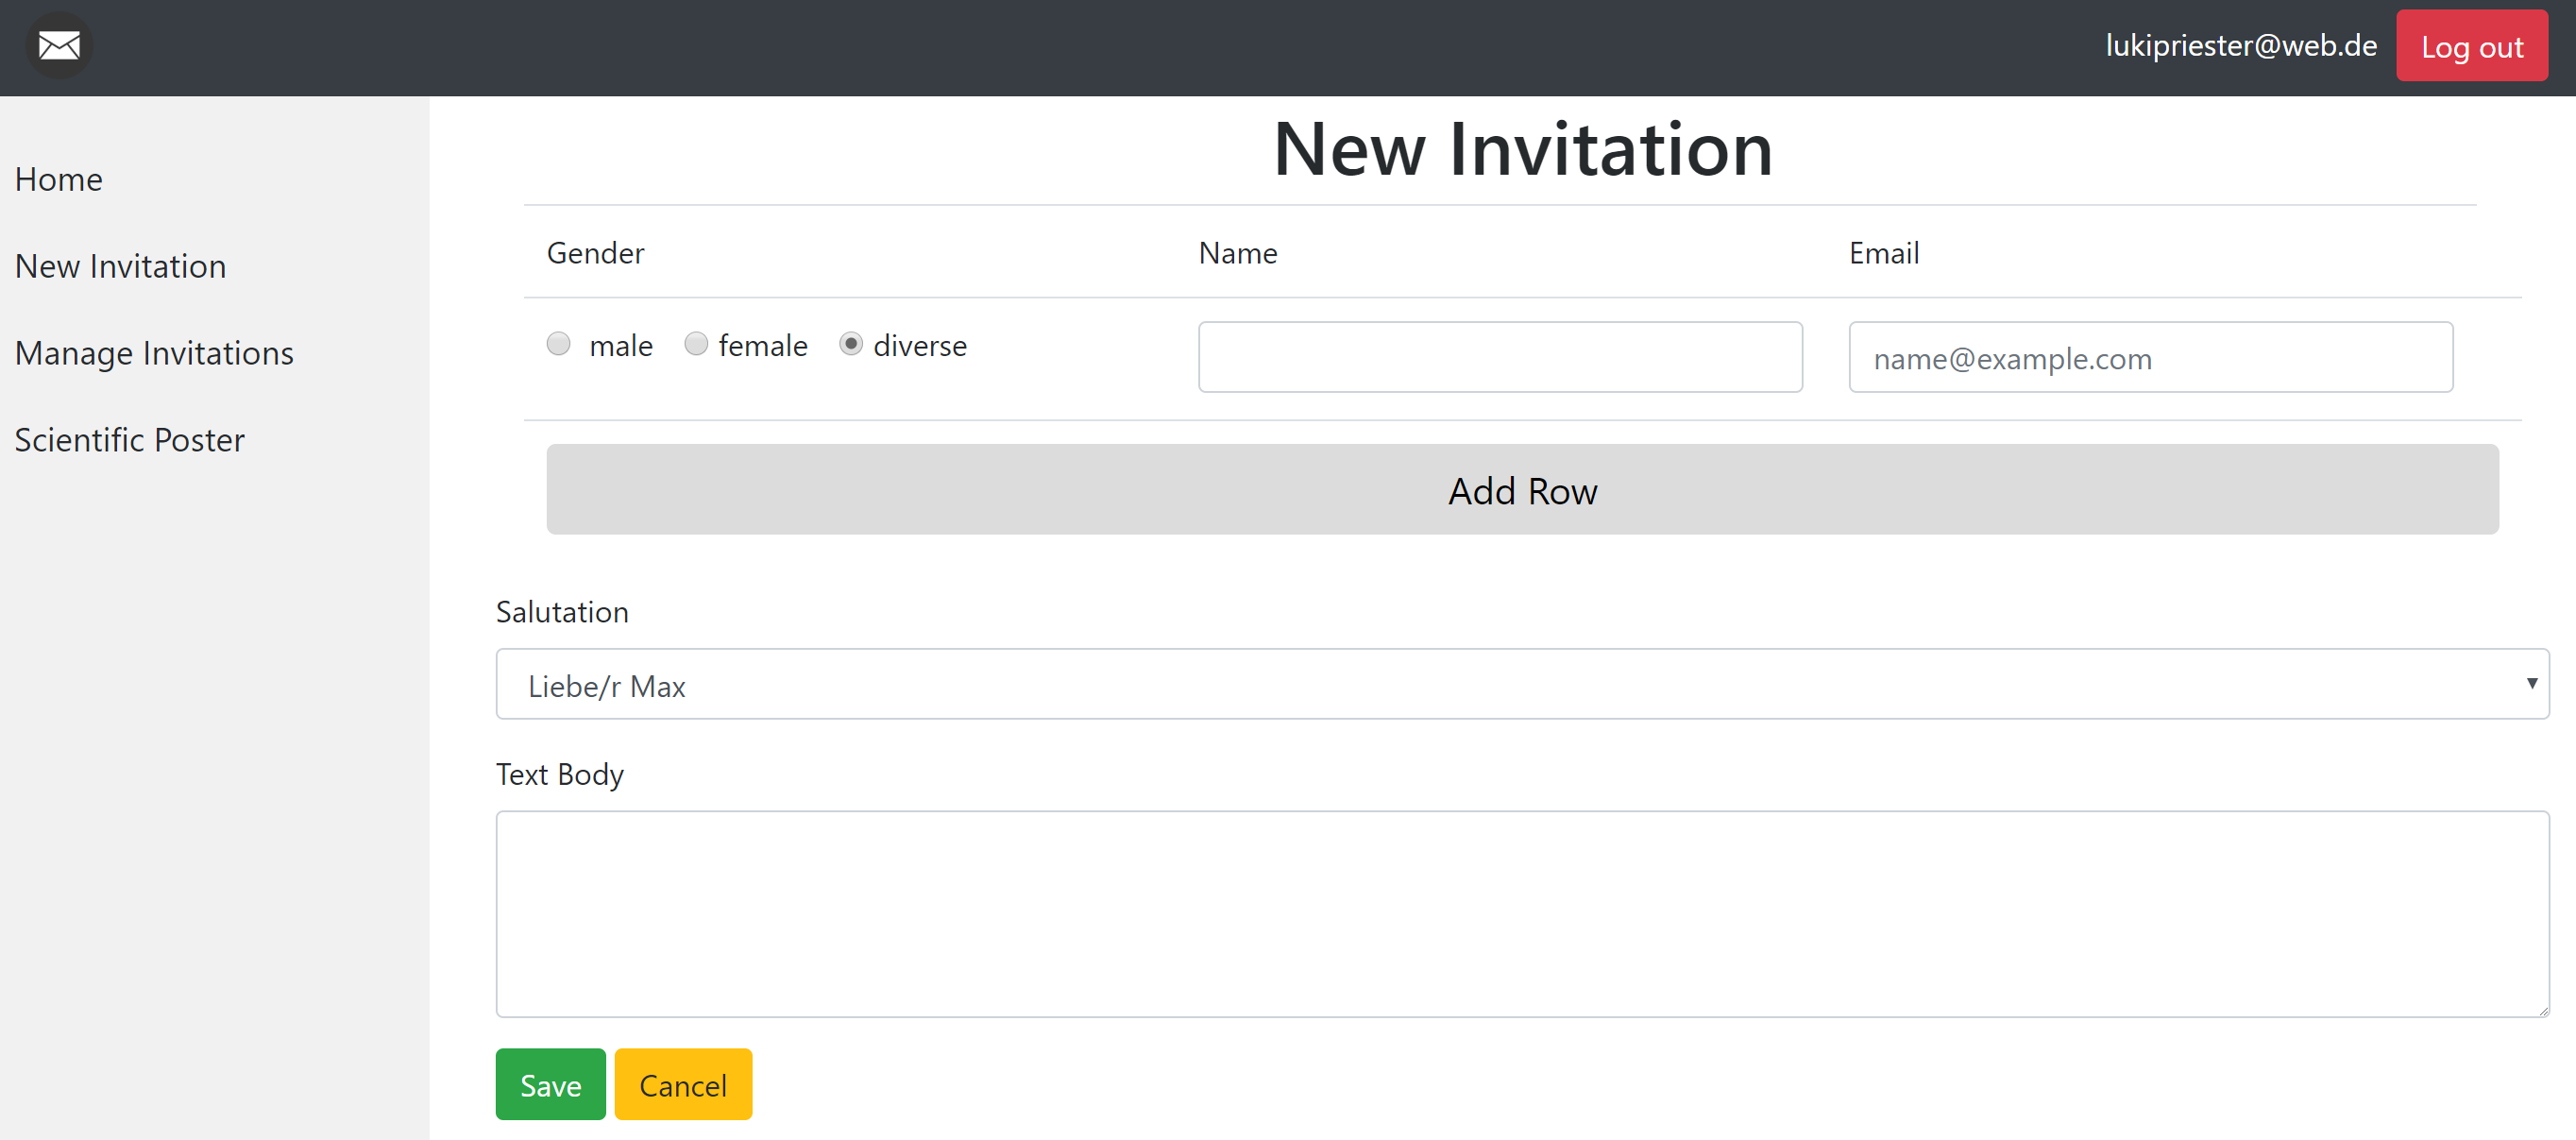
\includegraphics[width=0.65\linewidth]{New_Invitation_Seite.PNG}
			\captionof{figure}{Webseite für neue Einladungen}\label{page_sample}
		\end{center}
	\end{multicols}
}
\end{poster}
\end{document}